\documentclass[11pt,a4paper]{article}

\usepackage[utf8]{inputenc}
\usepackage[T1]{fontenc}
\usepackage{lmodern}
\usepackage{graphicx}
\usepackage{booktabs}
\usepackage{amsmath}
\usepackage{hyperref}
\usepackage{natbib}
\usepackage[margin=2.5cm]{geometry}
\usepackage{xcolor}
\usepackage{float}
\usepackage{multirow}
\usepackage{array}
\usepackage{tabularx}

\bibliographystyle{plainnat}

\title{When Free Executors Cost More:\\The Free-Executor Paradox in Iterative LLM Code-Repair Loops}
\author{Ken Imoto\\Propel-lab\\Tokyo, Japan\\\texttt{imoto@propel-lab.co.jp}\\\url{https://kenimoto.dev}}
\date{June 2026}

\begin{document}

\maketitle

\begin{abstract}
The canonical recipe for cost-aware agentic coding---``use a strong model to orchestrate, a cheap model to execute''---fails on every iterative code-repair task we measured. We call this the \emph{free-executor paradox}: when the executor is free at the token meter (a locally hosted Qwen 3.5-9B), the orchestrator's prompt-cached re-reads of the executor's returned summaries grow its own input volume by 1.4--5.3$\times$ over running Opus alone, and the structure becomes the \textbf{most expensive cloud configuration we tested}, not the cheapest. We support the claim with a controlled comparison of four configurations---Opus 4.7 solo, Opus orchestrating Qwen 3.5-9B (free executor), Opus orchestrating Haiku 4.5, and Haiku 4.5 solo---on three Python code-repair tasks (25-error breakage recovery, refactor, feature-add) over 40 trials with $n = 3$ successful runs per cell. Correctness is judged deterministically by \texttt{mypy + ruff + pytest} exit codes; no LLM grades the work. Beyond the paradox, we report two practitioner-level observations: (i)~Haiku solo is 5.5$\times$ cheaper than the cheapest cloud arm on the longest task, but pays a 25\% failure rate at our per-arm iteration cap; (ii)~when Opus does orchestrate, Opus + Haiku---not the free executor---ties Opus solo on the longest task and beats it narrowly on the refactor task. Our headline question is therefore \emph{not} ``which model is best,'' but ``under what task structure does the orchestrator's read-back cost amortize against the executor's per-token savings.'' We provide a harness, runners, and analysis that make this question reproducible on any codebase for about \$36.
\end{abstract}

\begin{center}
\fbox{\parbox{0.92\textwidth}{\centering
\textbf{Artifact} \quad
Code, raw trial data, figures, and the \LaTeX{} source of this paper are open at\\
\url{https://github.com/kenimo49/free-executor-paradox} \quad (MIT code, CC-BY 4.0 text). \\
Zenodo DOI: \emph{to be assigned on upload.}
}}
\end{center}

\section{Introduction}

A standard cost-control move in agentic coding is to put a strong, expensive model in charge of planning and reasoning, and to delegate the mechanical edits to a cheap or free executor. The intuition is unambiguous: the executor handles the bulk of the tokens, and the orchestrator only pays for the decisions. We show that this intuition breaks down in the \emph{iterative} regime that drives a deterministic judge to convergence, because the orchestrator is forced to re-read what the executor did on every subsequent iteration.

Most prior comparisons of orchestrated vs solo configurations are framed around \emph{query-level} routing or single-shot cascades. RouteLLM~\citep{ong2024routellm} routes individual queries; FrugalGPT~\citep{chen2023frugalgpt} cascades models on confidence. In both, the orchestrator's cost is paid once per user query. Agentic coding, by contrast, is iterative: the agent edits, runs the harness, reads the failure, edits again, often 20--90 times per task. The orchestrator's input grows with the trajectory, not with the query. To our knowledge, that growth has not been quantified against a deterministic judge in published work.

The field has settled on two informal heuristics for the iterative regime---``biggest model, every call'' and ``one cheap model, more retries''---neither of which is justified by direct comparison under a fair judge. Most published comparisons of agentic coding rely either on LLM-as-judge or on aggregate benchmarks (HumanEval, MBPP, SWE-bench), and neither captures the cost-iteration-correctness tradeoff faced by an agent that \emph{is allowed to retry until it converges}.

This paper makes three contributions:
\begin{enumerate}
    \item We use a \textbf{decision-deterministic} harness---three tools (mypy, ruff, pytest) whose exit codes alone constitute the correctness judgment. No LLM grades the work. This removes one common confounder from agentic-coding benchmarks.
    \item We add a ``\textbf{\$0 marginal cost executor}'' axis to the orchestration comparison, in the form of a locally hosted Qwen 3.5-9B model.
    \item We measure \textbf{iterations to convergence} as a primary metric alongside dollars and wall-time, giving budget-aware practitioners a directly actionable signal.
\end{enumerate}

The empirical result of our small experiment is that the canonical ``cheap-executor'' orchestration form (Opus + Qwen, arm B) does not pay off on any of the three tasks we tested. The mechanism is straightforward: with prompt caching, the orchestrator's cost is dominated by its own context, which grows with executor output volume even when executor tokens themselves are free.

\section{Related Work}

\paragraph{Query-level routing.}
\citet{ong2024routellm} routes individual queries between strong and weak models based on a learned classifier. Our setting differs structurally: we measure the \emph{full iterative loop} required to drive a deterministic judge to a green state, not a single query.

\paragraph{Cost-aware cascades.}
\citet{chen2023frugalgpt} chains models in a cheap-to-expensive cascade, accepting an answer at the first stage with high enough confidence. We compare a cascade-adjacent setup (Opus orchestrator + cheap executor) under a hard convergence requirement rather than a confidence threshold.

\paragraph{Multi-LLM collaboration.}
\citet{wang2024moa} aggregates outputs across multiple LLMs with LLM-judge synthesis. Our orchestrator-executor structure is functionally adjacent but uses a deterministic harness as judge.

\paragraph{Planner-executor agents.}
\citet{shen2023hugginggpt} and \citet{wang2023voyager} use planner-executor decompositions but do not measure per-trial dollar cost against a deterministic correctness oracle.

\paragraph{Code-change benchmarks.}
For evaluation context, \citet{jimenez2024swebench} grade agentic code changes against real-world repository tests. Our setup is a much smaller, controlled variant in which the same harness is reused across configurations rather than a benchmark suite of unseen problems. To our knowledge, we are not aware of a prior published comparison that combines (i)~Anthropic Opus vs Haiku on the same task harness, (ii)~a locally hosted ``free executor'' axis, and (iii)~a non-LLM judge.

\section{Method}

\subsection{Arms}

\begin{table}[H]
\centering
\begin{tabularx}{\textwidth}{l l l X}
\toprule
\textbf{arm} & \textbf{orchestrator} & \textbf{executor} & \textbf{role split} \\
\midrule
A & Opus 4.7 & (solo) & one model handles everything \\
B & Opus 4.7 & Qwen 3.5-9B (local, Ollama) & Opus plans + verifies, Qwen edits \\
C & Opus 4.7 & Haiku 4.5 & Opus plans + verifies, Haiku edits \\
D & Haiku 4.5 & (solo) & one cheap model handles everything \\
\bottomrule
\end{tabularx}
\caption{Four configurations under comparison. All call the Anthropic API through the SDK; arm B additionally calls Qwen via the \texttt{qwen-task --agent} wrapper.}
\end{table}

All four arms have access to identical tools: a \texttt{str\_replace\_editor} (view / create / str\_replace / insert) scoped to the typer repository root, and a \texttt{bash} tool with a 120-second timeout. Orchestrators (B, C) additionally have a \texttt{delegate\_to\_executor(instruction)} tool that hands a single concrete instruction string to the executor.

The orchestrator and executor see \textbf{slightly different system prompts}. The solo system prompt (A, D) lets the model freely use \texttt{str\_replace\_editor}. The orchestrator prompt asks the model to avoid editing directly and to delegate edits instead. This asymmetry is intentional---it is how a real orchestrator/executor split would be deployed---but it is also a confounder, since it shapes the orchestrator's behavior beyond just adding the delegate tool. We return to this in Section~\ref{sec:limitations}.

Anthropic prompt caching is enabled identically on every call: \texttt{system}, tool definitions, and the most recent user message are marked with \texttt{cache\_control: ephemeral}. No \texttt{temperature} or \texttt{seed} is set on either Anthropic or Qwen calls, so trial-to-trial variance reflects sampling stochasticity.

\subsection{Tasks}

All three tasks operate on the \texttt{typer}~\citep{ramirez2024typer} repository at tag \texttt{0.26.8} (commit \texttt{b210c0e}, MIT license). Each trial begins with \verb|git checkout -- . && git clean -fd typer/ tests/| to restore the base state. The base repository is cloned at experiment time, not vendored.

\paragraph{T1 --- Breakage recovery.}
A Python script using \texttt{ast.parse} deterministically injects 25 errors across 15 source / test files: 10 mypy type errors, 10 ruff lint errors, and 5 pytest collection-time failures (\texttt{assert False} lines prepended after the last top-level import in five test modules). The agent must return the harness to fully green.

\paragraph{T2 --- Refactor.}
Move the function \texttt{get\_params\_from\_function} from \texttt{typer/utils.py} to a new module \texttt{typer/\_param\_extractor.py}. Update every import site so that no file imports the function from the old location and at least one imports it from the new location. All tests must continue to pass.

\paragraph{T3 --- Feature-add.}
Implement \texttt{get\_version\_banner(prefix: str = "Typer", uppercase: bool = False) -> str}, re-export it from \texttt{typer/\_\_init\_\_.py}, and make it pass a provided test file. The test file is fingerprinted with SHA-256 at injection time; the verifier rejects any modification to it. We acknowledge that this fingerprinting biases T3 toward ``specification-following'' behavior over exploration.

\subsection{Harness}

A bash script runs \texttt{uv run mypy}, \texttt{uv run ruff check}, \texttt{uv run ruff format} (informational only, not a failure condition), and \texttt{uv run pytest} in sequence and emits a single JSON blob with per-tool counts. A green base on this harness takes 22 seconds and reports 1356 tests passing. T3 adds 3 expected passes. \texttt{verify-T2.sh} and \texttt{verify-T3.sh} add task-specific structural checks (e.g.\ function moved to new module, public API callable, fingerprinted test unchanged).

\subsection{Metrics}

Per trial, we record:
\begin{itemize}
    \item \textbf{success} --- verifier exit code = 0,
    \item \textbf{iterations} --- outer turns of the tool loop on the orchestrator side,
    \item \textbf{wall\_sec} --- seconds from \texttt{setup\_task} to verifier completion,
    \item \textbf{cost\_usd} --- tokens $\times$ public rate card (Opus 4.7: \$15 / \$75 per M input / output; Haiku 4.5: \$1 / \$5; cache write 1.25$\times$, cache read 0.10$\times$ of the input rate; Qwen marginal cost \$0),
    \item per-role token usage (input / output / cache\_write / cache\_read).
\end{itemize}

\subsection{Trial budget}
\label{sec:budget}

Per-arm outer-loop caps are a design variable, not a model property:

\begin{table}[H]
\centering
\begin{tabular}{lrrr}
\toprule
\textbf{arm} & \textbf{T1 cap} & \textbf{T2 cap} & \textbf{T3 cap} \\
\midrule
A & 40 & 40 & 40 \\
B & 80 & 60 & 60 \\
C & 40 & 40 & 40 \\
D & 100 & 120 & 80 \\
\bottomrule
\end{tabular}
\caption{Iteration caps per arm and task. D (Haiku solo) needs the highest cap because its per-iteration capability is lowest.}
\end{table}

Within these caps, failures count against the cell's success rate rather than being silently retried. We aim for $n \geq 3$ \emph{successful} trials per (arm, task) cell. Trials that exhaust the cap are recorded as failures and excluded from median statistics; their counts contribute to the visible success-rate column.

\subsection{Statistical procedure}

We report median and IQR per cell (success-only), and pairwise Mann-Whitney $U$ tests on the \texttt{cost\_usd} column within each task. Two-sided $p$-values use a normal approximation; under that approximation and $n = 3$--$4$ per cell, $p = 0.050$ is the boundary value. An exact Mann-Whitney $U$ would yield slightly different small-sample $p$; we read $p = 0.050$ here as ``as different as this sample size can show under this approximation'' rather than as a strong significance claim.

\section{Results}

\subsection{Summary table}

Table~\ref{tab:summary} reports per-cell success-only medians, the 95\% bootstrap confidence interval for cost, and a \emph{cost-per-success} column (median cost divided by success rate) that approximates expected cost under a retry-on-failure policy.

\begin{table}[H]
\centering
\small
\begin{tabular}{l l c r r r l r r}
\toprule
\textbf{arm} & \textbf{task} & \textbf{$n_{s}/n$} & \textbf{wall (s)} & \textbf{iters} & \textbf{cost (\$)} & \textbf{95\% CI} & \textbf{cost/succ} & \textbf{success} \\
\midrule
A Opus solo   & T1 & 3 / 3 & 253 & 36 & 1.74 & [1.24, 1.84] & 1.74 & 1.00 \\
A Opus solo   & T2 & 3 / 4 & 233 & 26 & 1.11 & [0.86, 1.14] & 1.48 & 0.75 \\
A Opus solo   & T3 & 3 / 3 & \textbf{69} & \textbf{6}  & 0.17 & [0.17, 0.43] & 0.17 & 1.00 \\
\midrule
B Opus+Qwen   & T1 & 3 / 4 & 484 & 38 & 2.27 & [2.05, 2.60] & 3.03 & 0.75 \\
B Opus+Qwen   & T2 & 3 / 3 & 443 & 27 & 1.38 & [1.20, 1.48] & 1.38 & 1.00 \\
B Opus+Qwen   & T3 & 3 / 3 & 348 & 12 & 0.42 & [0.42, 0.70] & 0.42 & 1.00 \\
\midrule
C Opus+Haiku  & T1 & 3 / 3 & 400 & \textbf{28} & 1.67 & [1.08, 2.07] & 1.67 & 1.00 \\
C Opus+Haiku  & T2 & 3 / 3 & 275 & \textbf{20} & \textbf{0.92}$^\dagger$ & [0.91, 1.43] & 0.92 & 1.00 \\
C Opus+Haiku  & T3 & 3 / 3 & 145 & 11 & 0.38 & [0.35, 0.43] & 0.38 & 1.00 \\
\midrule
D Haiku solo  & T1 & 3 / 4 & 758 & 89 & \textbf{0.30} & [0.19, 0.43] & 0.40 & 0.75 \\
D Haiku solo  & T2 & 3 / 4 & 507 & 70 & \textbf{0.23} & [0.23, 0.31] & 0.31 & 0.75 \\
D Haiku solo  & T3 & 3 / 3 & 208 & 29 & \textbf{0.08} & [0.07, 0.08] & 0.08 & 1.00 \\
\bottomrule
\end{tabular}
\caption{Success-only medians, bootstrap 95\% CI (10,000 resamples), and cost-per-success. Bolded numbers are per-task per-column winners. $^\dagger$ C is the cheapest \emph{cloud} arm on T2; D is cheaper overall but with a 25\% failure rate. Cell totals: 40 trials, total Anthropic spend \$35.98.}
\label{tab:summary}
\end{table}

\subsection{Pareto frontiers}

Figures~\ref{fig:pareto-t1}, \ref{fig:pareto-t2}, and \ref{fig:pareto-t3} show cost (USD) on the $x$-axis and wall-time (seconds) on the $y$-axis per task. Each arm contributes a colored cluster of trial dots and a square marker at the success-only median.

\begin{figure}[H]
\centering
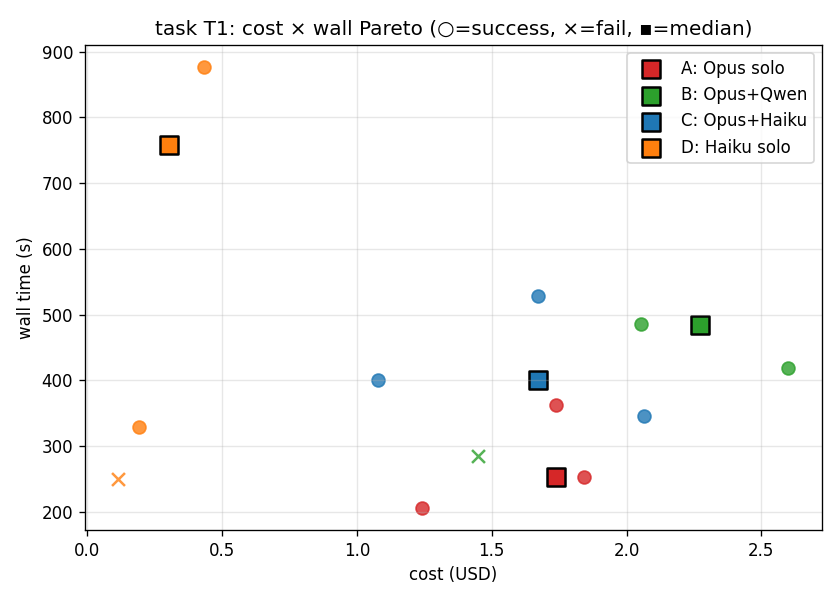
\includegraphics[width=0.80\textwidth]{../results/figures/pareto-T1.png}
\caption{T1 breakage-recovery Pareto. D holds the cost extreme; C takes over for cloud-only setups; A holds the wall-time extreme; B is dominated on both axes by C. One D, one A T2, one B T1, and one D T2 trial fail at the per-arm cap (shown as $\times$).}
\label{fig:pareto-t1}
\end{figure}

\begin{figure}[H]
\centering
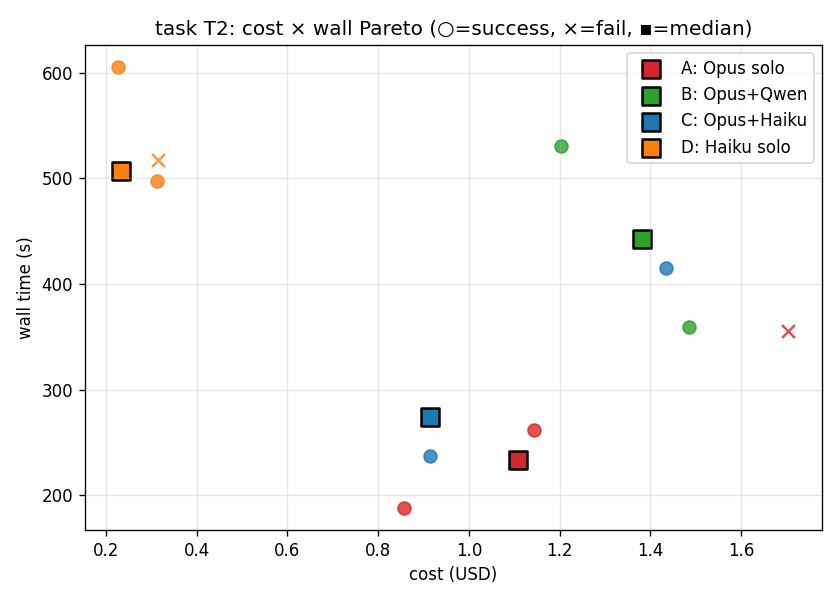
\includegraphics[width=0.80\textwidth]{../results/figures/pareto-T2.png}
\caption{T2 refactor Pareto. D and C anchor the frontier; A is on the frontier (faster than C); B is dominated.}
\label{fig:pareto-t2}
\end{figure}

\begin{figure}[H]
\centering
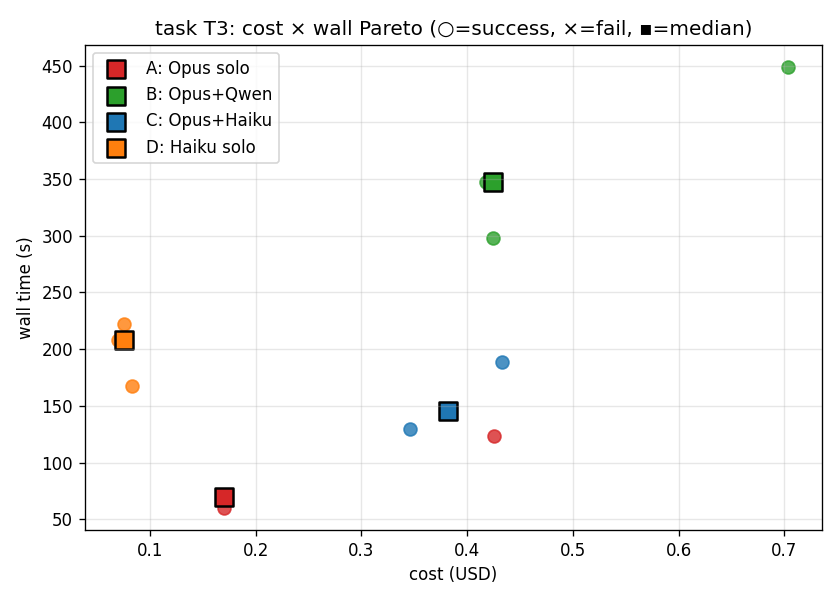
\includegraphics[width=0.80\textwidth]{../results/figures/pareto-T3.png}
\caption{T3 feature-add Pareto. Opus solo (A) at \$0.17 / 69 s is Pareto-dominant on wall-time and undominated except by Haiku solo on cost. B and C are both dominated by A on this task.}
\label{fig:pareto-t3}
\end{figure}

\subsection{Pairwise Mann-Whitney $U$ (cost) per task}

\begin{table}[H]
\centering
\small
\begin{tabular}{l r r r r r r}
\toprule
\textbf{task} & \textbf{A vs B} & \textbf{A vs C} & \textbf{A vs D} & \textbf{B vs C} & \textbf{B vs D} & \textbf{C vs D} \\
\midrule
T1 & 0.050 & 0.827 & 0.050 & 0.127 & 0.050 & 0.050 \\
T2 & 0.050 & 0.827 & 0.050 & 0.275 & 0.050 & 0.050 \\
T3 & 0.275 & 0.275 & 0.050 & 0.275 & 0.050 & 0.050 \\
\bottomrule
\end{tabular}
\caption{Two-sided $p$-values, normal approximation. Under this approximation and $n = 3$--$4$, $p = 0.050$ is the boundary value.}
\label{tab:mwu}
\end{table}

Under this approximation, we did not detect a cost difference between A and C on T1 and T2 ($p = 0.827$). D's cost is at the minimum observable $p$ ($= 0.050$) against every other arm on every task, but the small sample size limits the strength of this claim. B (Opus + Qwen) is at the same boundary $p$ versus A on T1 and T2, despite Qwen's tokens being free at the meter.

To complement Mann-Whitney $U$ under small $n$, Table~\ref{tab:cliffs} reports Cliff's delta~\citep{romano2006effect} on the cost column. The direction is read as ``how often does the row arm cost less than the column arm''---negative means row is cheaper. All comparisons of B against the cheaper arms (A on T1/T2, C, D) yield a \emph{large} positive delta, confirming that the rank ordering is not an artifact of one outlier trial.

\begin{table}[H]
\centering
\small
\begin{tabular}{l r r r r}
\toprule
\textbf{task} & \textbf{B vs A} & \textbf{B vs C} & \textbf{C vs A} & \textbf{D vs C} \\
\midrule
T1 & $+1.00$ (large) & $+0.78$ (large)  & $-0.11$ (negligible) & $-1.00$ (large) \\
T2 & $+1.00$ (large) & $+0.56$ (large)  & $+0.11$ (negligible) & $-1.00$ (large) \\
T3 & $+1.00$ (large) & $-0.11$ (neg.)   & $+1.00$ (large)       & $-1.00$ (large) \\
\bottomrule
\end{tabular}
\caption{Cliff's delta on cost (positive = row arm is more expensive than column arm). Effect-size labels follow~\citet{romano2006effect}: $|d| < 0.147$ negligible, $< 0.330$ small, $< 0.474$ medium, otherwise large.}
\label{tab:cliffs}
\end{table}

\subsection{The free-executor paradox}

Compare the per-arm Opus-side token volume \texttt{input + cache\_read\_input} across tasks (success-only median):

\begin{table}[H]
\centering
\begin{tabular}{l r r r}
\toprule
\textbf{arm role (Opus side)} & \textbf{T1} & \textbf{T2} & \textbf{T3} \\
\midrule
A (Opus solo)               & 534{,}586 & 226{,}474 & 13{,}320 \\
B (Opus orchestrating Qwen) & 733{,}142 & 313{,}914 & 62{,}864 \\
C (Opus orchestrating Haiku) & 421{,}622 & 159{,}640 & 44{,}016 \\
\bottomrule
\end{tabular}
\caption{Opus input + cache\_read tokens, success-only median.}
\label{tab:opus-tokens}
\end{table}

\begin{figure}[H]
\centering
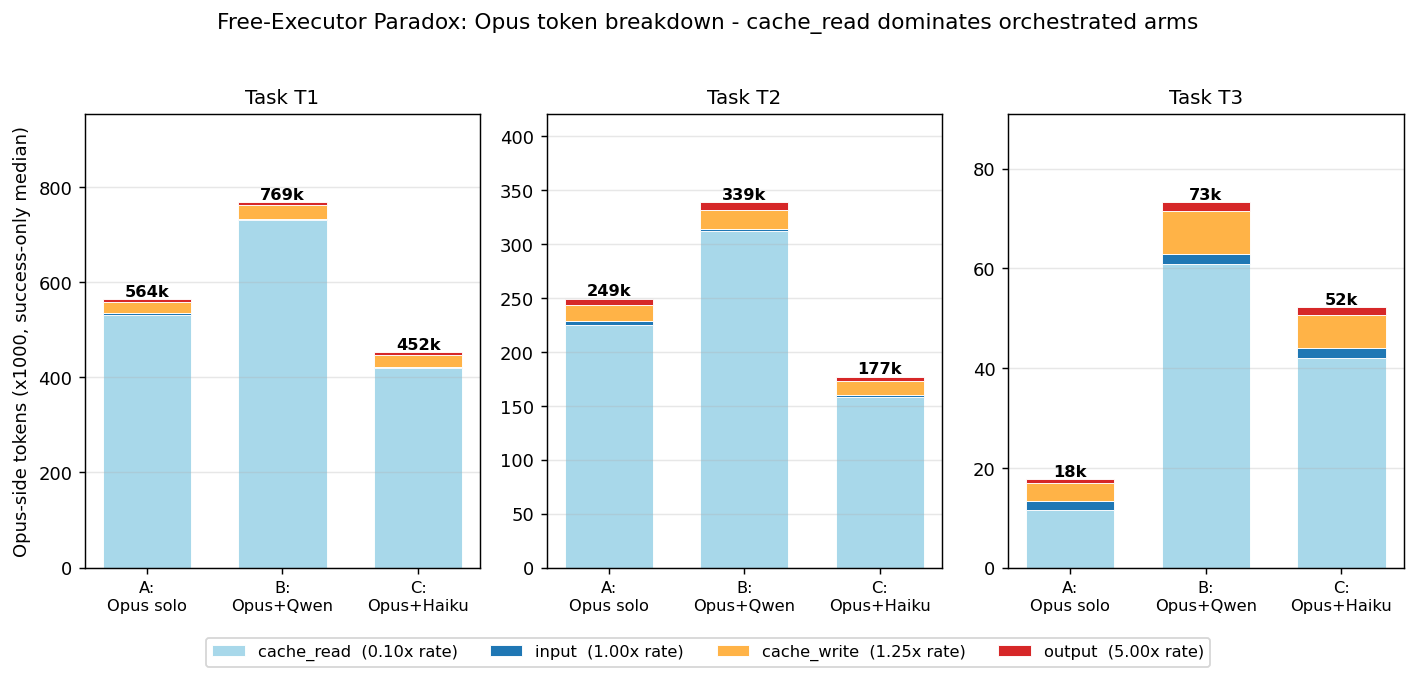
\includegraphics[width=0.92\textwidth]{../results/figures/token-growth.png}
\caption{Free-executor paradox visualized as a token-component breakdown. Each stacked bar is the success-only median of Opus-side tokens for one (task, arm) cell, decomposed into \texttt{cache\_read} (light blue, billed at 0.10$\times$ input rate), \texttt{input} (dark blue, 1.00$\times$), \texttt{cache\_write} (orange, 1.25$\times$), and \texttt{output} (red, 5.00$\times$). Two patterns: (i)~the dominant component is \texttt{cache\_read} (orchestrator re-reading prior turns), not new input or output; (ii)~arm B's bars are the tallest in every task, even though B's executor (Qwen) costs \$0 at the token meter.}
\label{fig:token-growth}
\end{figure}

\begin{figure}[H]
\centering
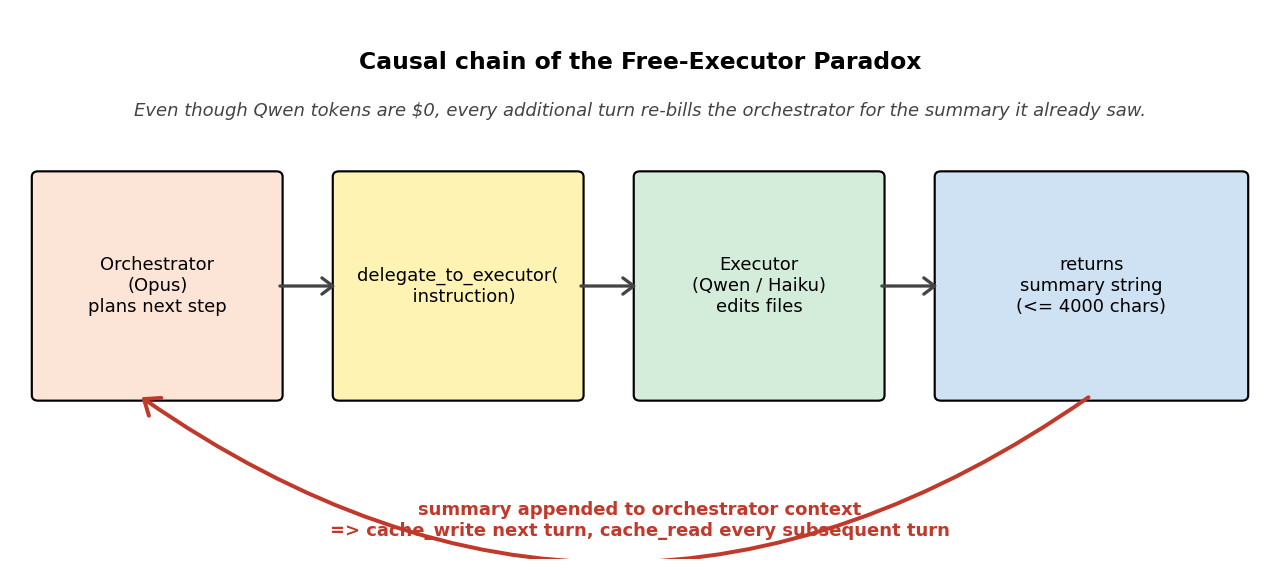
\includegraphics[width=0.85\textwidth]{../results/figures/mechanism.png}
\caption{Causal chain underlying the paradox. The orchestrator delegates an instruction, the executor edits files and returns a summary string, and that summary is appended to the orchestrator's context. On the \emph{next} turn that summary becomes a \texttt{cache\_write}; on every subsequent turn it becomes part of the \texttt{cache\_read} payload, re-billed at 10\% of the input rate per iteration. Over 30--80 iterations of T1 this loop pays for the entire executor delegation many times over.}
\label{fig:mechanism}
\end{figure}

The B-over-A ratio of \texttt{cache\_read} alone is \textbf{1.38$\times$ on T1, 1.39$\times$ on T2, and 5.26$\times$ on T3}. Even though B's executor (Qwen) is free, the orchestrator side of B reads back more cache tokens per iteration than Opus solo. Two observations follow.

First, the multiplier is largest on T3, the smallest task. The base context (system + tools + initial prompt) is amortized across iterations; on long tasks (T1, T2) it is a smaller fraction of total input, so the orchestration overhead is less visible. On short tasks, the overhead dominates.

Second, C (Opus + Haiku) sees a \emph{smaller} \texttt{cache\_read} footprint than A (Opus solo) on T1 and T2 (0.79$\times$ and 0.70$\times$ of A). The executor in C does substantive work that Opus would otherwise have to do itself, and the executor's \emph{summary} (not its full output) is what flows back into Opus.

The mechanism is therefore not ``executor outputs free $\to$ orchestrator reads them all.'' It is ``executor outputs summary $\to$ orchestrator reads summary, and on small tasks the summary is large relative to the base.'' This is consistent with our observed cost ordering: B is most expensive on T3 (where the multiplier is 5.3$\times$), and only modestly more expensive than A on T1 (where the multiplier is 1.4$\times$).

\section{Discussion}

\subsection{Why orchestration loses on dollars in our setup}

In a one-shot routing setup such as RouteLLM, the orchestrator's only cost is the routing decision; the chosen model bears the answer-generation cost alone. In an iterative tool loop, however, the orchestrator must read whatever the executor returns through its \texttt{delegate\_to\_executor} tool---in our implementation, that is a truncated stdout summary (Qwen, up to 4000 chars) or the executor's final text (Haiku, up to 1500 chars), not the executor's full intermediate output. Even so, that returned summary accumulates in the orchestrator's context across 30--80 iterations on T1 and feeds into \texttt{cache\_write} and \texttt{cache\_read} on every subsequent turn.

A free executor's ``free'' applies only to that executor's own tokens. The orchestrator's cost grows in proportion to how much it must \emph{re-read} about what the executor did, not how much the executor itself produced.

\subsection{When orchestration would win}

Our setup does not reproduce the regimes in which orchestration is most likely to pay:
\begin{itemize}
    \item Executors whose returned summaries are tightly bounded---e.g.\ one structured diff, not free-form prose. Our \texttt{qwen-task --agent} wrapper does not enforce that.
    \item Tasks with many independent sub-problems that can run in parallel under one orchestration. Our three tasks are inherently sequential within a single trial.
    \item Repeated trials in which the orchestrator can amortize its cache across runs. We reset the harness between trials, so each trial pays its own \texttt{cache\_write}.
\end{itemize}

A reasonable next experiment would constrain executor return size to a few hundred tokens per delegation and rerun arm B; we expect the gap to A to narrow, and perhaps invert on T3 specifically.

\subsection{The cost-reliability tradeoff}

The cost ordering D $\ll$ C $\approx$ A $<$ B is qualified by reliability. D's per-trial cost advantage on T1 (\$0.30 vs C \$1.67, ratio 5.5$\times$) is bought at a 25\% failure rate within our per-arm iteration cap. For a CI pipeline that retries failed runs, the expected cost is roughly $\mathit{cost\_med} / \mathit{success\_rate}$; D's \emph{expected} T1 cost becomes \$0.40, narrowing the cloud-vs-Haiku gap from 5.5$\times$ to 4.2$\times$. For a human in the loop who pays for failed runs as time, the gap is wider.

The right model choice is a function of the cost of failure recovery, not just of median cost per trial.

\subsection{Performance differs across task types}

T3 (feature-add) requires about 6 iterations of edit-test-edit. Within that small budget, Opus's per-iteration efficiency pays for itself: A is undominated on wall-time, iterations, and cloud-only cost simultaneously. T1 (25-error recovery) requires 30--90 iterations regardless of model; here Haiku's lower per-iteration cost dominates the dollar axis, and C---sharing cheap iteration-time costs between Opus and Haiku---is the cheapest cloud-only arm. T2 sits between the two on iteration count, and C narrowly wins the cloud-only cost axis (\$0.92 vs A's \$1.11).

These three task types are not points along a single ``complexity'' axis we have measured. They differ in iteration count, in the structural specificity of the verifier, and in how much the agent is rewarded for spec-reading versus exploration. We describe the result as ``varies across task types'' rather than as ``rotates with complexity.''

The practical guidance we are willing to give is narrower: \textbf{use the cheaper-per-iteration model when the task requires many iterations, and consider orchestration when the executor's returned summary can be tightly bounded}---neither of which our arm B reliably delivers.

\section{Threats to Validity}
\label{sec:limitations}

We organize threats to validity along the standard software-engineering empirical-research axes~\citep{wohlin2012experimentation}: internal validity (do the results follow from the experiment as designed), external validity (do they generalize beyond it), and construct validity (does the measurement capture what we claim).

\subsection{Internal Validity}

\begin{itemize}
    \item \textbf{Sampling non-determinism.} We did not pin \texttt{temperature} or \texttt{seed} on any Anthropic or Qwen call. Reported variance is sampling-driven and partly an artifact of API defaults. Within-cell variance is non-trivial: A T3 iterations were 6 / 6 / 16, and C T2 iterations were 17 / 20 / 36.
    \item \textbf{Iteration cap as design variable.} The per-arm cap (Section~\ref{sec:budget}) is set by the experimenter. Failures within budget would become successes given a larger cap. The success-rate column reflects cap policy, not pure model capability.
    \item \textbf{System-prompt asymmetry between solo and orchestrator arms.} A and D's prompts let them edit freely; B and C's orchestrator prompts ask them to avoid direct edits and delegate instead. This is faithful to deployment but is a confounder for any ``structure alone'' comparison.
    \item \textbf{Statistical strength.} With $n = 3$ successful trials per cell, the minimum two-sided Mann-Whitney $p$ under normal approximation is $0.050$. The Cliff's-delta complement (Table~\ref{tab:cliffs}) helps but does not replace larger $n$.
\end{itemize}

\subsection{External Validity}

\begin{itemize}
    \item \textbf{Single repository.} All three tasks are scoped within \texttt{typer} v0.26.8. Whether the free-executor paradox extends to larger codebases (e.g.~\texttt{httpx}, \texttt{click}, \texttt{fastapi}) is future work. We expect the qualitative direction to hold because the mechanism (orchestrator re-reads of executor summaries through prompt cache) is repository-independent, but the magnitude should grow with longer task trajectories.
    \item \textbf{Two cloud models.} We compare Anthropic Opus 4.7 and Haiku 4.5 only. Sonnet, GPT-class models, and Gemini are absent.
    \item \textbf{One local executor.} Qwen 3.5-9B is the only local model tested. A 30B-class local model would shift wall-time and possibly executor capability, but not dollar cost.
    \item \textbf{No parallel sub-task structure.} Our three tasks are sequential within a single trial. We do not measure regimes where multiple delegate calls could fan out concurrently, which would shift the orchestrator's amortization profile.
\end{itemize}

\subsection{Construct Validity}

\begin{itemize}
    \item \textbf{Test fingerprinting (T3).} SHA-256 fingerprinting of the T3 test file biases T3 toward spec-following behavior over exploration. The conclusion ``Opus solo dominates on T3'' should be read as ``on spec-following tasks of T3's size,'' not as ``on all small tasks.''
    \item \textbf{The harness itself.} \texttt{mypy + ruff + pytest} exit code $= 0$ is one correctness oracle. Code-review quality, security, and maintainability are not measured here.
    \item \textbf{Executor summary as proxy for executor output.} The orchestrator never sees the executor's raw work; it sees a truncated summary returned by the \texttt{delegate\_to\_executor} tool. This is how real orchestrator-executor systems are deployed, but it means our paradox quantifies summary read-back, not raw output transfer.
\end{itemize}

\subsection{Threat Matrix}

Table~\ref{tab:threats} summarizes the threats above, the headline claim each touches, and the mitigation already in place or proposed.

\begin{table}[H]
\centering
\small
\begin{tabular}{p{3.4cm} l p{3.5cm} p{4.5cm}}
\toprule
\textbf{Threat} & \textbf{Type} & \textbf{Headline impact} & \textbf{Mitigation in place / proposed} \\
\midrule
Sampling non-determinism & Internal & Within-cell variance & report 95\% bootstrap CI (Table~\ref{tab:summary}); future: pin temperature \\
Iteration cap & Internal & Success rate column & report cost-per-success and CI; future: $n \times 2$ at next cap \\
Prompt asymmetry (solo vs orch.) & Internal & Cross-arm comparability & document explicitly (\S\ref{sec:budget}); future: symmetric ablation \\
Small $n$ ($=3$) & Internal & p-value floor at 0.050 & Cliff's delta (Table~\ref{tab:cliffs}) to complement; future: scale $n \to 10$--$20$ \\
Single repository & External & Generalization & mechanism is repo-independent (\S5.1); future: \texttt{httpx}, \texttt{click}, \texttt{fastapi} \\
Two cloud models & External & Vendor specificity & cache mechanism is vendor-specific but the structural argument is not; future: GPT-5, Gemini 2 \\
One local executor & External & Executor-LLM specificity & paradox argument relies on summary-volume, not on Qwen; future: 30B-class local \\
No parallel delegation & External & Amortization regime & sequential trial structure documented; future: parallel-fanout extension \\
T3 SHA-256 fingerprint & Construct & T3 specifically & limit T3 claim to spec-following; future: open-spec variant \\
Harness as oracle & Construct & Code quality unmeasured & we claim correctness only, not maintainability; future: LLM-judge complement \\
Summary as proxy for output & Construct & Mechanism scope & we measure summary read-back, not raw output; future: enforce summary $\leq$ 500 tokens \\
\bottomrule
\end{tabular}
\caption{Threat matrix. ``Mitigation in place'' refers to the current paper; ``proposed'' is deferred to future work (\S\ref{sec:future}).}
\label{tab:threats}
\end{table}

\section{Future Work}
\label{sec:future}

The mechanism we report has at least four extensions that we view as the most useful next experiments, in roughly increasing cost order.

\paragraph{1. Bounded-summary executors.}
The orchestrator's cache_read footprint grows with the size of the executor's returned summary. Replacing free-form \texttt{stdout} returns with structured summaries capped at a few hundred tokens (e.g. a JSON diff, a unified-format patch, or a single sentence) should shrink the B/A ratio toward 1.0$\times$ and potentially invert it on T3. We expect this to be the cheapest experiment to run on the existing harness.

\paragraph{2. Larger repositories.}
Replicating the 4-arm $\times$ 3-task design on \texttt{httpx}, \texttt{click}, and \texttt{fastapi} would address the external-validity gap directly. The mechanism predicts the paradox should hold and that the dollar gap should \emph{widen} on longer trajectories, because cache\_read is the dominant term. A counter-finding (no paradox on \texttt{fastapi}, say) would be diagnostic of repository structure, not of the mechanism.

\paragraph{3. Additional model families.}
Adding Sonnet 4.6 (between Opus and Haiku in capability and cost) tests whether the paradox is a property of strong-vs-weak pairing in general or specifically of Opus--Haiku. GPT-5 and Gemini 2 (when stable cache pricing is published) extend the test across vendors. We expect the qualitative pattern to hold because prompt caching has converged across vendors, but the precise multipliers depend on rate-card structure.

\paragraph{4. Parallel orchestration.}
The current design is strictly sequential within a trial. A parallel delegation regime---multiple \texttt{delegate\_to\_executor} calls fanned out per orchestrator turn---would shift the orchestrator's amortization profile, because the orchestrator pays the cache cost \emph{once} for $k$ executor calls instead of $k$ times. This is the most architecturally different extension and the one most likely to surface a regime where arm B wins.

We also intend to mirror the harness on \texttt{cargo check + cargo test} for Rust and on \texttt{go vet + go test} for Go, to verify the mechanism is not a Python-specific artifact.

\section{Conclusion}

We did not set out to declare a winner. We set out to ask whether the cost gap between ``use Opus everywhere'' and ``use Opus to orchestrate something cheap'' is large enough to justify the extra plumbing.

For our particular cheap-executor instantiation---Opus orchestrating local Qwen 3.5-9B (arm B)---the answer is \emph{no on every task we tested}. The mechanism is straightforward: prompt-cached orchestration re-reads the executor's returned summary on every iteration, so an executor that is ``free'' at the token meter is not free at the orchestrator's input.

The picture is more nuanced for Opus + Haiku (arm C), which beats Opus solo on the cloud-only dollar axis for T2 and ties it for T1. Within the cloud, ``orchestrate when the executor is also a competent reasoner'' is a defensible heuristic; ``orchestrate so the executor can be free'' is not in our setup.

The contribution we hope is most reusable is the methodology, not the verdict. A harness-judged comparison cost about \$36 of API time and a few hours of wall-clock to produce twelve cells of Pareto data on a real codebase. The numbers should be small enough for practitioners to run their own comparisons on their own codebases.

\section*{Reproducibility}

Tested on Ubuntu 22.04 with Python 3.10+ (typer requires \verb|>=3.10|), \texttt{uv} 0.4+, and \texttt{anthropic} Python SDK 0.83+. The Qwen executor uses Ollama 0.4+ on a Tailscale-reachable host running model \texttt{qwen3.5:9b}, exposed via the \texttt{qwen-task --agent} wrapper from \texttt{iris-hub}.

\begin{verbatim}
# 1. Clone iris-lab + go to experiment dir
git clone https://github.com/kenimo49/iris-lab
cd iris-lab/experiments/025-orchestrator-vs-solo

# 2. Clone base repo (typer at 0.26.8, commit b210c0e)
git clone --depth 1 --branch 0.26.8 \
    https://github.com/tiangolo/typer base-repo/typer
(cd base-repo/typer && uv sync)

# 3. Confirm green base on the harness
./harness.sh --json-only   # expect exit_code=0, 1356 passed

# 4. Provide ANTHROPIC_API_KEY (env or iris-lab/.env)
export ANTHROPIC_API_KEY=...

# 5. (Optional) point at Ollama host for arm B
export OLLAMA_HOST=http://<tailscale-host>:11434

# 6. Run a single trial end-to-end
python -m runners.runner --arm A --task T3 --trial 0

# 7. Full re-run targeting n=3 successes/cell
./runners/batch.sh all 3

# 8. Regenerate tables + Pareto plots
python3 analysis/analyze.py --plot
python3 analysis/export_csv.py
\end{verbatim}

For arm B specifically: if Ollama / Tailscale are unavailable, arm B trials will time out at the delegate-tool boundary; arms A, C, D remain runnable.

\section*{Acknowledgements}

The \texttt{typer} project (Sebastián Ramírez et al., MIT) provided the substrate. The Qwen team open-sourced the model used in arm B. The Codex CLI from OpenAI was used to perform an independent read-only review of this manuscript prior to revision; review records are linked from the GitHub issue tracker.

\bibliography{references}

\appendix

\section{System prompts}
\label{app:system-prompts}

All four arms use prompts of the same surface form; the only differences are whether \texttt{delegate\_to\_executor} is mentioned and whether direct editing is encouraged. We include them verbatim because the asymmetry is a confounder we discuss in \S\ref{sec:limitations}.

\subsection{Solo prompt (arms A and D)}

\begin{verbatim}
You are a code-fixing agent operating in a sandboxed Python repository.

You have two tools:
- `str_replace_editor`: view / create / str_replace / insert files
  (paths are repo-relative).
- `bash`: run shell commands in the repo root (120s timeout).

You will be given a task. Iteratively read code, run the harness, fix
issues, and re-run until the harness is green. Be concise in your
reasoning; spend tokens on tool calls, not narration.

When you believe the task is complete and the verifier passes, output a
single line `DONE` and stop. If you cannot make progress, output
`BLOCKED: <reason>` and stop.
\end{verbatim}

\subsection{Orchestrator prompt (arms B and C)}

\begin{verbatim}
You are the orchestrator of a two-LLM team. You decide WHAT to do; an
executor LLM (which can read files, edit files, and run shell commands)
does it for you.

You have three tools:
- `bash`: run shell commands in the repo root.
- `str_replace_editor`: read files yourself with `view` when you need to
  inspect something before instructing the executor. Avoid using
  create/str_replace -- delegate edits to the executor.
- `delegate_to_executor`: hand off a concrete edit/refactor instruction
  to the executor. The executor returns a short summary of what it did.
  Be precise: name files, name functions, name the exact change. The
  executor is cheaper but weaker than you, so spell out the change
  rather than asking it to "figure it out".

Loop: read harness output -> plan -> delegate small chunks -> check
harness -> repeat until green. Output `DONE` when verifier passes,
`BLOCKED: <reason>` if stuck.
\end{verbatim}

\subsection{Executor prompt (arm C only; arm B uses qwen-task default)}

\begin{verbatim}
You are an execution sub-agent. Another LLM (the orchestrator) has
handed you a concrete instruction. Do exactly what it asks using
`str_replace_editor` and `bash`. Do not expand scope. When done, output
`DONE: <one-line summary>` and stop. If the instruction is impossible
as written, output `BLOCKED: <reason>` and stop.
\end{verbatim}

\section{Harness output schema (sample)}
\label{app:harness}

\texttt{harness.sh --json-only} emits the following structure on a green base (\texttt{exit\_code = 0}):

\begin{verbatim}
{
  "exit_code": 0,
  "elapsed_sec": 22,
  "mypy":         {"exit": 0, "errors": 0},
  "ruff_check":   {"exit": 0, "errors": 0},
  "ruff_format":  {"exit": 0, "errors": 0, "informational": true},
  "pytest":       {"exit": 0, "passed": 1356, "failed": 0,
                   "collection_errors": 0}
}
\end{verbatim}

\texttt{exit\_code} is the only field the runner consumes for the gate (0 = pass). Per-tool counts are recorded for diagnostics and end up in the per-trial JSONL.

\texttt{verify-T2.sh} and \texttt{verify-T3.sh} wrap \texttt{harness.sh} and add task-specific structural checks (function moved to new module, public API callable, fingerprinted test unchanged); they emit the same outer schema with an extra \texttt{t2\_checks} or \texttt{t3\_checks} block.

\section{Per-trial JSONL schema}
\label{app:trial-schema}

Each trial appends one JSON object to \texttt{data/results/\{arm\}.jsonl}:

\begin{verbatim}
{
  "arm": "C", "task": "T1", "trial": 0,
  "success": true, "blocked": false,
  "wall_sec": 400.4, "iterations": 18,
  "usage_by_role": {
    "claude-opus-4-7": {
      "input_tokens": 2050, "output_tokens": 3803,
      "cache_creation_input_tokens": 17089,
      "cache_read_input_tokens": 170101
    },
    "claude-haiku-4-5-20251001": {
      "input_tokens": 15765, "output_tokens": 9774,
      "cache_creation_input_tokens": 62382,
      "cache_read_input_tokens": 435940
    }
  },
  "cost_usd_by_role": {
    "claude-opus-4-7": 0.891545,
    "claude-haiku-4-5-20251001": 0.186206
  },
  "total_cost_usd": 1.077752,
  "verify_final": {
    "exit_code": 0,
    "summary": "exit_code=0, mypy errors=0, ruff errors=0, "
               "pytest passed=1356 failed=0 collection_errors=0"
  }
}
\end{verbatim}

The 40 trials reported in this paper live in \texttt{data/results/\{A,B,C,D\}.jsonl} and the flattened table is at \texttt{data/trials.csv}.

\end{document}
